\documentclass[tikz]{standalone}
\usepackage{pgfplots}
\pgfplotsset{compat=1.15}
\usepackage{mathrsfs}
\usetikzlibrary{arrows,calc}
\usepackage{tkz-euclide}
\pagestyle{empty}

\definecolor{AngleClr}{rgb}{0,0.39215686274509803,0}
\definecolor{ShapeClr}{rgb}{0.6,0.2,0}
\definecolor{BlueSqr}{RGB}{5,81,163}
\definecolor{RedSqr}{RGB}{0, 156, 0}

\begin{document}

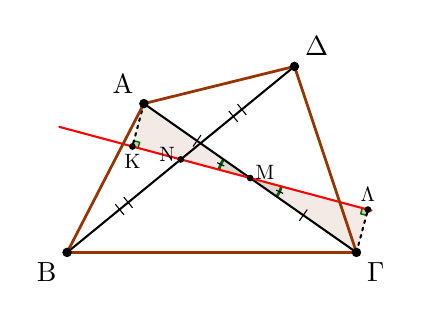
\begin{tikzpicture}[scale=.75]
\tkzSetUpLine[line width=1pt,color=black]
\tkzSetUpPoint[fill=black]

\tkzDefPoints{3.85/3.15/D,4.9/0/C,1.3/2.52/A,0/0/B}
\tkzFillPolygon[fill=white](A,B,C,D)


\tkzDefMidPoint(A,C) \tkzGetPoint{M}
\tkzDefMidPoint(B,D) \tkzGetPoint{N}

\tkzDefPointBy[projection=onto M--N](A)\tkzGetPoint{K}
\tkzDefPointBy[projection=onto M--N](C)\tkzGetPoint{L}

\tkzFillPolygon[fill=ShapeClr,fill opacity=0.1](M,K,A)
\tkzFillPolygon[fill=ShapeClr,fill opacity=0.1](M,L,C)

\tkzMarkRightAngles[line width=0.5pt, size=.1,color=AngleClr,fill=AngleClr,fill opacity=0.2](M,K,A M,L,C)

\tkzFillAngles[fill=AngleClr,size=.55,fill opacity=0.1](A,M,K C,M,L)
\tkzMarkAngles[mark=|,mksize=1.4,line width=1pt,size=.55,color=AngleClr](A,M,K C,M,L)

\tkzDrawSegments[line width=0.75pt,color=black](A,C B,D)
\tkzDrawSegment[line width=0.75pt,color=red,add=1.75 and 1.75](M,N)
\tkzDrawSegments[line width=0.75pt,color=black,dashed,dash pattern=on 1pt off 1.75pt](A,K C,L)

\tkzDrawPolygon[color=ShapeClr](A,B,C,D)
\tkzDrawPoints[size=3](A,B,C,D)
\tkzDrawPoints[size=2](M,N,K,L)
\tkzLabelPoint[above left](A){$\rm A$}
\tkzLabelPoint[below left](B){$\rm B$}
\tkzLabelPoint[below right](C){$\rm \Gamma$}
\tkzLabelPoint[above right](D){$\rm \Delta$}

\tkzLabelPoint[scale=0.75,below](K){$\rm K$}
\tkzLabelPoint[scale=0.75,above](L){$\rm \Lambda$}

\node[scale=0.75,yshift=0.09cm, xshift=0.25cm] at (M) {$\rm M$};
\node[scale=0.75,yshift=0.09cm, xshift=-0.23cm] at (N) {$\rm N$};

\tkzMarkSegments[mark=|,size=2.5](A,M M,C)
\tkzMarkSegments[mark=||,size=2.5](B,N N,D)


\end{tikzpicture}

\end{document}
